\tma{6.1 [Pitágoras]} Para todo triángulo rectángulo $\angle ABC$ con $\angle A$ recto, se tiene que $$BC^2 = AC^2+ AC^2$$
\begin{figure}[H]
	\centering
	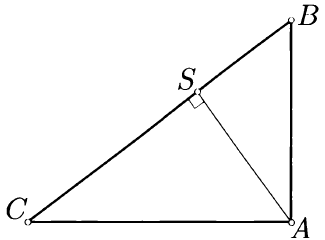
\includegraphics[width=3.5cm]{figuras/6-1.png}
	\vspace{-1em}
\end{figure}
\obligatorio\dem{Consideramos el punto $S\in r_{BC}$ tal que $r_{SA}\perp r_{CB}$. Pese a que es evidente, hay que demostrar que $S\in[B,C]$. Observamos que $SC < CA < BC$, la primera igualdad por $\cos \angle C = \frac{SC}{CA} < 1 \iff SC < CA$. Del mismo modo, $BS < BC$. Entonces, $S\in [B,C]$.\linebreak
Ahora observamos que
$$\cos \angle C = \frac{CA}{CB} = \frac{CS}{CA}$$
Por otra parte, también vemos que 
$$\cos \angle B = \frac{BS}{AB} = \frac{AB}{BC}$$
De ambas expresiones tenemos que (1) $CA^2 = CB\cdot CS$ y (2) $AB^2 = BS\cdot BC$. Así, $CB\cdot CS + CB\cdot BS = CB(CS+BS) = CB^2 = CA^2 + BA^2$.
}

\cor{6.3} Sea $\angle C$, entonces $$\sen^2 \angle C + \cos^2 \angle C = 1$$  

\dem{Si tenemos que $BC = 1$, entonces $\cos \angle C = \frac{CA}{CB}  = CA$ y $\sen \angle C = \frac{BA}{BC} = BC$. Aplicando el teorema de Pitágoras, entonces $ \sen^2 \angle C + \cos^2 \angle C =  BA^2 + CA^2 = BC^2 = 1$.} 

\tma{6.4} Dado $x \in [0, \pi] \subset \R$, existe un ángulo $\angle V$ tal que $\measuredangle V = x$.

\tma{6.5}  $\angle P = \angle Q$ sii $\measuredangle P = \measuredangle Q$

\defi{6.6} Sea $\triangle ABC$ y $h_B \perp r_{CA}$ y que pasa por $B$, y sea el punto $P_{h,b}$ el punto de corte de $h_B$ y $r_{CA}$. Entonces, $P_{h,b}$ es el \textbf{pie de la altura de $B$}, y $[P_{h,b},B]$ es la \textbf{altura} de $\triangle ABC$ desde $B$.
\begin{figure}[H]
	\centering
	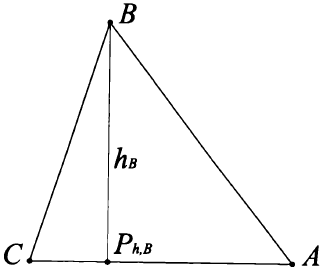
\includegraphics[width=3.5cm]{figuras/6-6.png}
	\vspace{-1em}
\end{figure}

\tma{6.7} En el triángulo de la \defi{6.6}, si $\angle A$ y $\angle C$ son agudos, entonces $P_{h,b} \in [C,A]$. Si $\angle A$ o $\angle C$ es obtuso, entonces $P_{h,b} \not\in [C,A]$.

\tma{6.8 [Fórmula del coseno]} Sea $\triangle ABC$ un triángulo, entonces se cumple que $$BC^2 = AB^2 + AC^2 - 2\cdot AB \cdot AC \cdot \cos \angle A$$
\dem{Basándonos en la figura de la \defi{6.6}, y por el \tma{6.7} [en el caso de $\triangle$ acutángulo], entonces se forman dos triángulos rectángulos $\triangle P_{hB}BC$ y $\triangle P_{hB}BA$ donde se verifica que $CA = CP_{hB} + P_{hB}A$
Por el \tma{de Pitágoras} tenemos que
$$AB^2 = P_{hB}A^2 + P_{hB}B^2 \qquad BC^2 = BP_{hB}^2+P_{hB}C^2$$
Si sustituimos una igualdad en otra tenemos que 
$$BC^2 = CP_{hB}^2 + AB^2 - P_{hB}A^2$$
Como $CA = CP_{hB} + P_{hB}A$ entonces
$$BC^2 = (CA - P_{hB}A)^2 + AB^2 - P_{hB}A^2 = $$
$$CA^2  \textcolor{SkyBlue}{+P_{hB}A^2} - 2\cdot CA\cdot P_{hB}A  + AB^2  \textcolor{SkyBlue}{-P_{hB}A^2}$$
Si quitamos las partes en azul, y consideramos que $P_{hB}A = AB\cos\angle A$, entonces queda el teorema demostrado.}

\cor{6.9} Dado un triángulo donde $BC^2 = AB^2 + AC^2$ entonces es un triángulo rectángulo, con $\angle A$ recto. 
\dem{Si aplicamos el \tma{del coseno}, entonces, el término $ 2\cdot AB \cdot AC \cdot \cos \angle A = 0$, y como $AB \neq 0, AC \neq 0$, entonces $\cos \angle A = 0 \iff \angle A$ es recto (\tma{6.5}).} 

\tma{6.10 [Fórmula de los senos]} Sea $\triangle ABC$, entones se verifica
$$\frac{AB}{\sen \angle C} = \frac{AC}{\sen \angle B}  = \frac{BC}{\sen \angle A}$$
\dem{Seguimos con la figura de la \defi{6.6}. Vemos que $BP_{hB} = BC\sen \angle C = BA\sen\angle A$. Si el triángulo es obtusángulo también se cumple porque los senos se mantienen.
Simplemente, igualando $BP_{hB}$ tenemos que $\frac{BC}{\sen \angle A} = \frac{BA}{\sen \angle C}$. El resto de igualdades se consiguen con las demás alturas.}

\tma{6.11}  Para $\triangle ABC$...
\begin{itemizex}
	\item Si se conoce $\measuredangle A$ y $AB, AC$ (adyacentes), entonces se pueden hallar $\measuredangle B, \measuredangle C, BC$. 
	\item Si se conocen $AB, AC, BC$ entonces se pueden hallar $\measuredangle A, \measuredangle B, \measuredangle C$.
	\item Si se conocen $AB, \measuredangle A, \measuredangle B$ entonces se pueden hallar $BC, AC, \measuredangle C$.
\end{itemizex}

\cor{6.12 [Criterios de congruencia de $\triangle$]} Dados $\triangle ABC$ y $\triangle A'B'C'$ entonces
\begin{itemizex}
	\item $\measuredangle A =  \measuredangle A', AB = A'B', AC = A'C'$ [LAL]
	\item $AB = A'B', AC = A'C', BC = B'C'$ [LLL]
	\item $\measuredangle A = \measuredangle A', \measuredangle B = \measuredangle B', AB = A'B'$ [ALA]
\end{itemizex}
Entonces existe una isometría $\eta$ tal que $\eta(A) = A'$, etc. y $\triangle ABC = \triangle A'B'C'$. Hay que considerar que para emplear isometrías pares hay que definir la orientación de los triángulos.

\cor{6.14} Sean $\angle P$ y $\angle Q$ no nulos, y sumables. Entonces
$$ \sen(\angle P  + \angle Q) = \sen(\angle P)\cos(\angle Q) + \sen(\angle Q)\cos(\angle P) $$
$$ \cos(\angle P  + \angle Q) = \cos(\angle P)\cos(\angle Q) - \sen(\angle P)\sen(\angle Q)$$

\cor{6.15} Sean  $\angle P$ y $\angle Q$ no nulos, y sumables. Entonces 
$$\measuredangle (\angle P  + \angle Q) = \measuredangle P + \measuredangle Q$$
\dem{Nota: en el punto final se demuestra que $$\cos(\angle P + \angle Q) = \cos(\measuredangle P + \measuredangle Q)$$
Sabiendo que $\measuredangle P = \arccos(\cos \angle P)$
entonces $\arccos(\cos(\angle P +\angle Q)) = \measuredangle(\angle P + \angle Q)$ y, por tanto,
$$ \measuredangle(\angle P + \angle Q) = \arccos(\cos(\measuredangle P + \measuredangle Q)) = \measuredangle P + \measuredangle Q$$}
\cor{6.16} Si $\angle V$ es un ángulo y $n$ es entero, entonces existe $n\angle V$ y $\measuredangle (n \angle V) = n \measuredangle V$.

\ej{6.10} El centro de Fermat, $F$ es aquel que minimiza la distancia a los vértices del triángulo. Este sucede cuando el ángulo entre dos vértices cualesquiera del triángulo y $F$ es $2\pi/3$.


